\documentclass{article}

\usepackage{graphicx}
\usepackage{tikz}
\usepackage{tikzsymbols}
\usetikzlibrary{calc,patterns,shapes.geometric}
\pagestyle{empty}
\usepackage[margin=0pt]{geometry}
\geometry{papersize={14in,12in}}

\def\centerarc[#1](#2)(#3:#4:#5){\draw[#1] ($(#2)+({#5*cos(#3)},{#5*sin(#3)})$) arc (#3:#4:#5);}

\begin{document}
	\begin{figure}
		\centering
		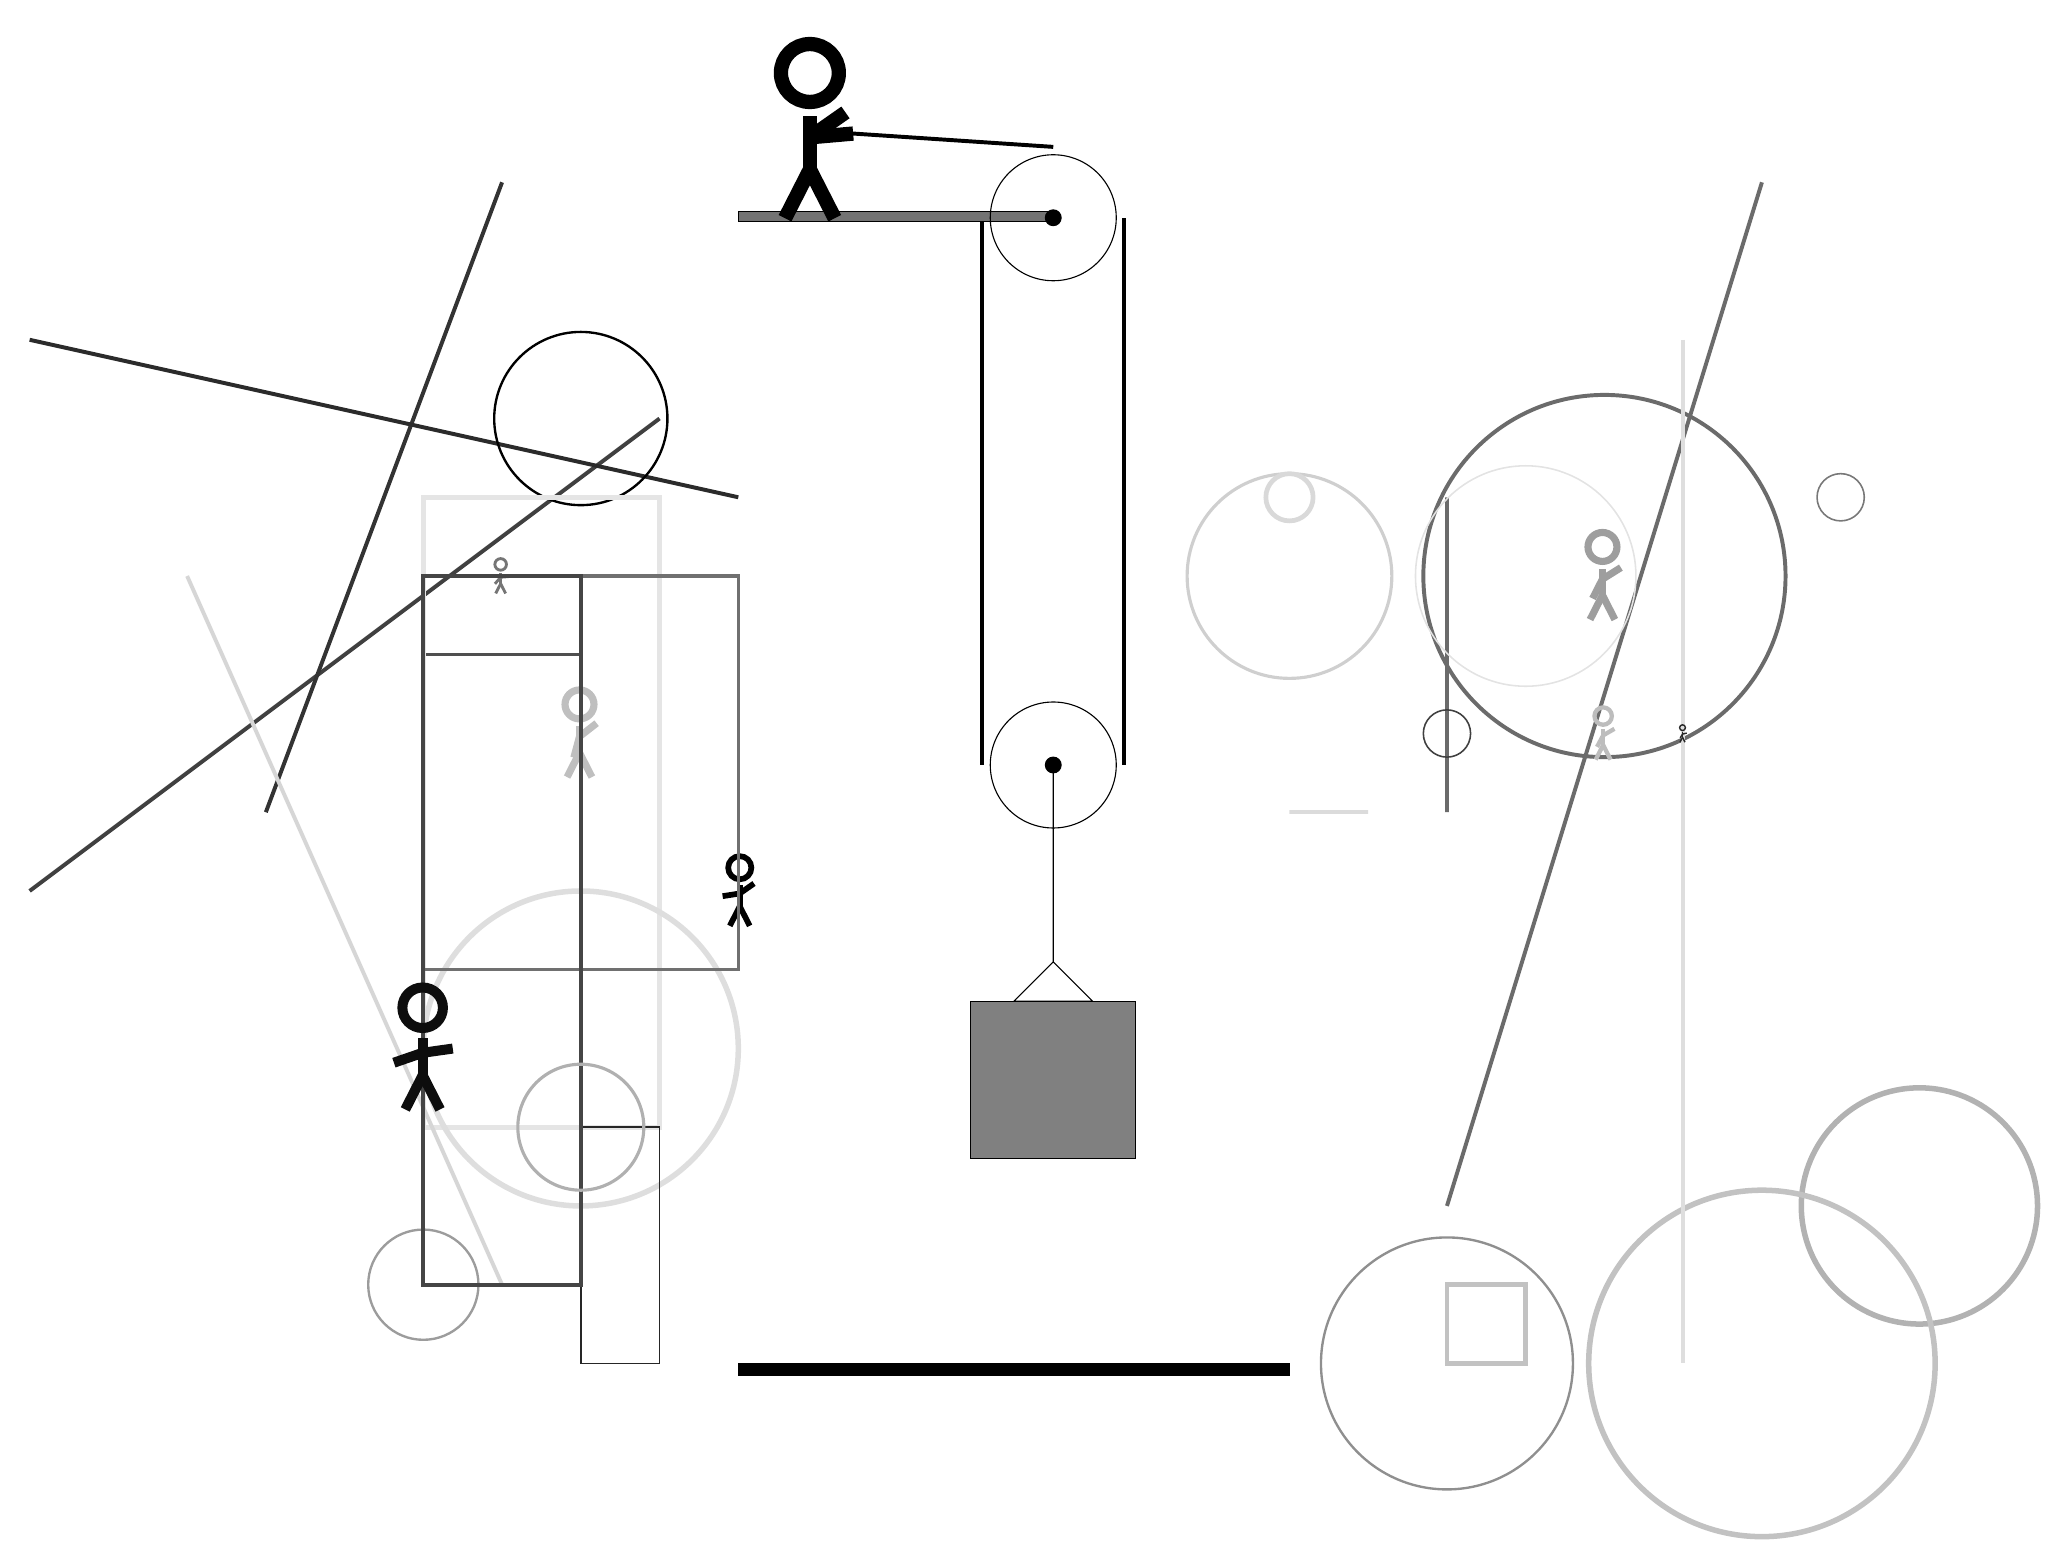
\begin{tikzpicture}
			%%%%% START %%%%%
			
			\draw[fill=black!55] (-2, 11.5) rectangle (2, 11.625);
			
			\draw (2, 4.6) circle (0.8);
			\draw[fill=black] (2, 4.6) circle (0.1);
			
			\draw (2, 11.55) circle (0.8);
			\draw[fill=black] (2, 11.55) circle (0.1);
			
			\draw (2, 4.6) -- (2, 2.1) -- (1.5, 1.6) -- (2.5, 1.6) -- (2, 2.1);
			\draw[fill=black!50] (0.95, 1.6) rectangle (3.05, -0.4);
			
			\draw[line width=0.6mm, color=black!58] (7, 4) rectangle (7, 8);
			
			\draw[line width=0.5mm, color=black!75](-3, 9) -- (-11, 3);
			\draw [line width=0.5mm, color=black!58](9, 7) circle (2.3);
			\draw[line width=0.4mm, color=black!69] (-4, 6) rectangle (-6, -2);
			
			\draw[line width=0.5mm, color=black!80](-5, 12) -- (-8, 4);
			\draw [line width=0.7mm, color=black!30](13, -1) circle (1.5);
			
			\draw[line width=0.5mm, color=black!58](7, -1) -- (11, 12);
			\draw[line width=0.6mm, color=black!24] (7, -3) rectangle (8, -2);
			\draw [line width=0.3mm, color=black!44](7, -3) circle (1.6);
			\draw [line width=0.4mm, color=black!19](5, 7) circle (1.3);
			\draw[line width=0.5mm, color=black!83](-2, 8) -- (-11, 10);
			\node[line width=0.5mm, color=black!100] at (-2, 3) {\Strichmaxerl[4][9][35]};
			\draw [line width=0.7mm, color=black!24](11, -3) circle (2.2);
			\draw [line width=0.2mm, color=black!75](7, 5) circle (0.3);
			\draw [line width=0.3mm, color=black!100](-4, 9) circle (1.1);
			\draw[line width=0.6mm, color=black!10] (-3, 8) rectangle (-6, 0);
			
			\draw [line width=0.3mm, color=black!39](-6, -2) circle (0.7);
			\draw [line width=0.7mm, color=black!13](-4, 1) circle (2.0);
			\draw [line width=0.2mm, color=black!11](8, 7) circle (1.4);
			\draw [line width=0.2mm, color=black!53](12, 8) circle (0.3);
			\draw[line width=0.2mm, color=black!85] (-4, -3) rectangle (-3, 0);
			\draw[line width=0.5mm, color=black!13](10, 10) -- (10, -3);
			\node[line width=0.4mm, color=black!54] at (-5, 7) {\Strichmaxerl[2][49][5]};
			\node[line width=0.4mm, color=black!84] at (10, 5) {\Strichmaxerl[1][58][14]};
			\draw[line width=0.5mm, color=black!16](-5, -2) -- (-9, 7);
			
			\node[line width=0.4mm, color=black!25] at (-4, 5) {\Strichmaxerl[5][75][38]};
			\draw[line width=0.5mm, color=black!14] (6, 4) rectangle (5, 4);
			\draw[line width=0.4mm, color=black!56] (-2, 7) rectangle (-6, 2);
			\draw [line width=0.6mm, color=black!15](5, 8) circle (0.3);
			
			\node[line width=0.5mm, color=black!38] at (9, 7) {\Strichmaxerl[5][63][32]};
			\draw[line width=0.5mm, color=black!73] (-4, -2) rectangle (-6, 7);
			
			\draw [line width=0.4mm, color=black!31](-4, 0) circle (0.8);
			\node[line width=0.6mm, color=black!26] at (9, 5) {\Strichmaxerl[3][62][30]};
			\node[line width=0.5mm, color=black!95] at (-6, 1) {\Strichmaxerl[7][19][8]};
			
			
			\draw[line width=0.5mm] (1.1, 11.5) -- (1.1, 4.6);
			\centerarc[line width=0.5mm](2, 4.6)(180:360:0.9);
			\draw[line width=0.5mm](2.9, 4.6) -- (2.9, 11.55);
			\centerarc[line width=0.5mm](2, 11.55)(0:90:0.9);
			\draw[line width=0.5mm](2, 12.45) -- (-1, 12.65);
			
			\node at (-1, 12.65) {\Strichmaxerl[10][-175][35]};
			
			\draw[fill=black] (-2, -3) rectangle (5, -3.15);
			
			%%%%% END %%%%%
		\end{tikzpicture}
	\end{figure}	
\end{document}